\chapter{Organisation de l'équipe}
Cette partie a pour but de présenter les différents rôles de l'équipe projet que nous avons constituée. Pour chacun des rôles, nous présenterons leurs attributions.

\section{Chef de projet~: Valentina~\textsc{Zantedeschi}}
Chargée de la planification et de l'organisation, elle est également garante de la coordination et de la cohésion du groupe.

Elle effectuera le \textbf{suivi stratégique} du projet en évaluant les risques et en s'assurant du respect des objectifs dans les délais impartis. Elle veillera au bon \textbf{pilotage opérationnel} en planifiant les tâches et en les encadrant. Elle mettra tout en œuvre pour garantir une \textbf{organisation humaine} efficace en définissant le rôle de chacun des membres, en leur attribuant des tâches et en résolvant les éventuels conflits. Enfin, elle s'assurera du bon \textbf{pilotage de la production}, en suivant les résultats et les livrables.

\section{Responsable qualité~: Marina~\textsc{Julien}}
D'une manière générale, elle veillera à la \textbf{qualité des livrables} fournis au client. Elle s'assurera également de la cohésion entre les livrables, de la maintenance et du \textbf{respect du Plan d'Assurance Qualité}.

\section{Expert méthode et outils~: Thierry \textsc{Cantenot}}
Il sera chargé de \textbf{conseiller}, d'\textbf{assister}, de \textbf{former} et d'\textbf{informer}. Il effectuera également la \textbf{veille technologique} quant aux outils utilisés et \textbf{proposera des évolutions} qu'il juge nécessaires.

\section{Expert métier~: Guillaume \textsc{Abadie}}
Il enrichira l'équipe de sa connaissance métier de l'entreprise \texttt{SPI} et, par sa fine compréhension, permettra l'adéquation de la solution conçue aux besoins de l'entreprise. Il est le référent par excellence au sein de notre équipe pour toutes les questions à propos de l'entreprise \texttt{SPI}.


\section{Expert ERP~: Ahmed~\textsc{Kachkach}}
Assisté de ses collègues, possédant une expérience précieuse en solutions ERP, sa mission principale sera d'être le point d'appui de l'équipe pour l'\textbf{analyse} et la \textbf{conception} de l'\textbf{architecture générale}, ainsi que pour la \textbf{modélisation} et la \textbf{configuration} des \textbf{solutions} ERP.

\section{Responsable communication~: Martin~\textsc{Wetterwald}}
Canal de communication principal, il sera l'interface privilégiée entre l'équipe et les clients, en plus de garantir une bonne communication intra-équipe. Il sera le premier à être contacté par les clients en cas de problème avec les livrables (difficulté de transmission ou non-validation de la part du client).

\section{Histogramme des charges}
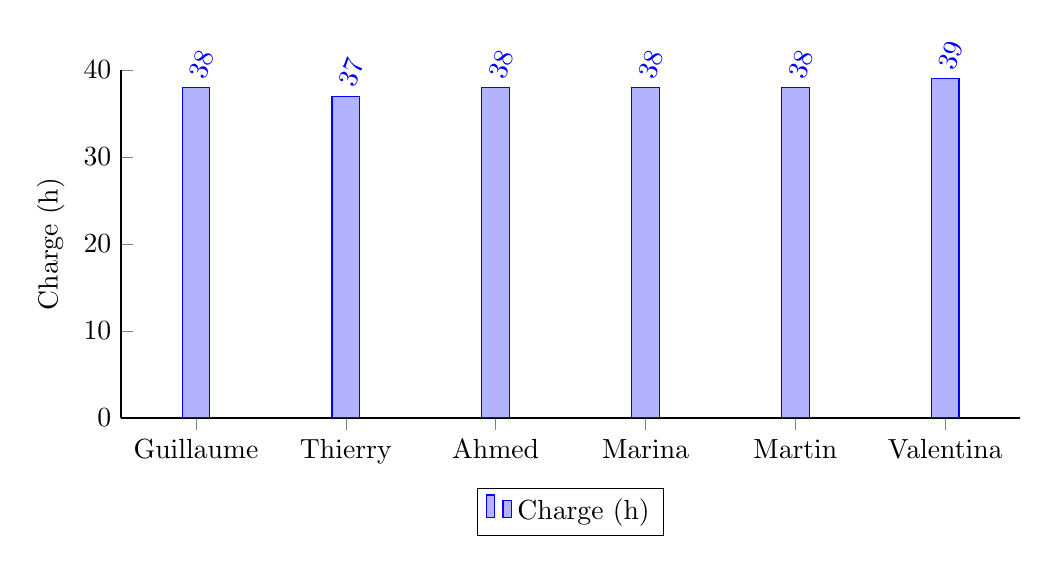
\begin{tikzpicture}
  \centering
  \begin{axis}[
	ybar,
    height=6cm,
    width=13cm,
    enlarge y limits=false,
    axis lines*=left,
    ymin=0,
    ymax=40,
     legend style={at={(0.5,-0.2)},
        anchor=north,legend columns=1},
		ylabel={Charge (h)},
        symbolic x coords={Guillaume,Thierry,Ahmed,Marina,Martin,Valentina},
     xtick=data,
        nodes near coords,
    every node near coord/.append style={
        anchor=mid west,
        rotate=70
    }
    ]
	\addplot coordinates {(Guillaume,38) (Thierry,37) (Ahmed,38) (Marina,38) (Martin,38) (Valentina,39)};
  \legend{Charge (h)}
  \end{axis}
\end{tikzpicture}
